\documentclass[10pt]{article}
\usepackage{graphicx,amssymb, amstext, amsmath, epstopdf, booktabs, verbatim, gensymb, geometry, appendix, natbib, lmodern}
\geometry{letterpaper}
%\usepackage{garamond}

\newcommand*\Title{Neurowrx Account Manual}
\newcommand*\cpiType{some subtitle}
\newcommand*\Date{Novermber 2018}
\newcommand*\Author{Michael Braeutigam}
\title{Neurowrx Account Manual}
\author{Michael Braeutigam}
\date{\today}
%-----------------------------------------------------------

\usepackage{cpistuff/cpi} % This is what makes your document look like a cpi document.


\begin{document}

\begin{titlepage}
\maketitle
\end{titlepage}

\linespread{1.15} %Set standard document linespacing

\begin{executive}

This is a document describing this template.

\frame{
\textbf{Key Findings}

After careful analysis, a number of conclusions have been reached:
\begin{enumerate}
	\item \textbf{This template works okay.}  But there are some minor hiccups and inelegant features.
	\item \textbf{Your feedback will help it to improve}  So please provide it.
	\item \textbf{Once it works well, formatting will not be a concern if you use \LaTeX.} This is the goal.
\end{enumerate}

These findings are based on an econometric study that uses the fact that state governments have implemented building codes at varying times to isolate the impact of building codes from underlying time trends, state characteristics, shifts in climate and prices, and economic conditions.  This strategy means that the findings described above cannot be attributed to nationwide trends or individual state characteristics that might otherwise lead to inaccurate conclusions.}
\end{executive}



\section{Text Tricks}

This section describes some custom CPI commands.

\subsection{Orange writing}

Use the \texttt{callout} command:

\callout{By the shores of gitchee gumee\\ by the shining big sea waters \\ stood the wigwam of Nokomis \\ brother of the moon, Nokomis.}

\subsection{Writing in a box}

Use the \texttt{frame} command:

\frame{ 'Twas brillig and the slithy toves did gyre and gimble in the wabe \\ all mimsy were the borogroves, and the mome raths outgrabe. \\ Beware the Jabberwock, my son, the claws that bite, the jaws that snatch \\ Beware the Jubjub bird, and shun the frumious Bandersnatch.}

\section{Presenting data}

This describes more general stuff.  If you are experienced with \LaTeX, you may already know this.

\subsection{Figures}
\begin{figure}[h]
\centering
\caption{This is a fat horse}
\label{fathorse}
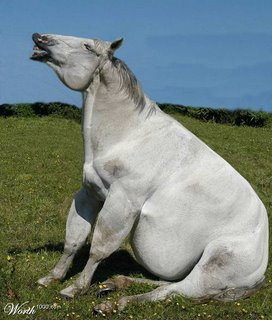
\includegraphics[scale=.5]{images/Fat+Horse.jpg}
\end{figure}

Figure \ref{fathorse} shows a fat horse.  You might use a more informative graphic.  If you make it in excel, make sure the dimensions are right before you export it, or it will be fuzzy.  I do that, and then copy it into paint and save it as a *.png (or *.jpg).  For Stata graphics, you can either save them as vector graphics (*.eps) and use \texttt{epstopdf} or save them as a normal graphic.  The advantage of vector graphics is that you can scale them without fuzziness.

\section{Ordinary Members}

Once access to th

\bibliography{codes_impact}
\bibliographystyle{plainnat}

\end{document}